\section{Data Mapping Directives}

\subsection{{\tt nodes} Directive}

The {\tt nodes} directive declares the name of a node set and its shape. A
node set can have a multi-dimensional shape.

\subsubsection{One-dimensional Node Set}

\begin{XCexample}
#pragma xmp nodes p[4]
\end{XCexample}

\begin{XFexample}
!$xmp nodes p(4)
\end{XFexample}

The nodes directive declares 1-dimensional node set p which has four
nodes. In XMP/C, the node set consists of p[0], p[1], p[2], and p[3]. In
XMP/Fortran, the node set consists of p(1), p(2), p(3), and p(4).

\subsubsection{Multi-dimensional Node Set}

\begin{XCexample}
#pragma xmp nodes p[2][3]
\end{XCexample}

\begin{XFexample}
!$xmp nodes p(3,2)
\end{XFexample}

The nodes directive declares 2-dimensional node set p which has six
nodes. In XMP/C, the node set consists of p[0][0], p[0][1], p[0][2],
p[1][0], p[1][1], and p[1][2]. In XMP/Fortran, the node set consists of
p(1,1), p(2,1), p(3,1), p(1,2), p(2,2), and p(3,2).

\begin{mynote}
  The ordering of the elements in a node set depends on the base
  language, C and Fortran. 
\end{mynote}

\subsubsection{Dynamic Node Set}

\begin{XCexample}
#pragma xmp nodes p[*]
\end{XCexample}

\begin{XFexample}
!$xmp nodes p(*)
\end{XFexample}

An asterisk symbol can be used in the nodes directive to declare a
dynamic node set. The program declares one-dimensional dynamic node set
p by using an asterisk symbol. The size of a dynamic node set is
determined at runtime (at the beginning of the execution). For example,
when the user runs the sample program with three nodes, the node set p
will have three nodes.

The user also can declare multi-dimensional dynamic nodes with an
asterisk symbol.

\begin{XCexample}
#pragma xmp nodes p[*][3]
\end{XCexample}

\begin{XFexample}
!$xmp nodes p(3,*)
\end{XFexample}

When the user runs the sample program with 12 nodes, the node set p will
have a shape of [4][3] in C, and (3,4) in Fortran.

\begin{mynote}
The user can use only one asterisk symbol in the last dimension of the node set.
\end{mynote}

\begin{myhint}
The dynamic node set may interfere with compiler optimizations. Static
node sets may achieve better performance in general.
\end{myhint}

\subsubsection{Partial Node Set}

The user can declare a partial node set from the existing node
set. Partial node sets can be used to optimize inter-node communication
by reducing the number of nodes participating in the communication.

\begin{XCexample}
#pragma xmp nodes p[16]
#pragma xmp nodes q[8]=p[0:8]
#pragma xmp nodes r[4][2]=p[8:8]
\end{XCexample}

\begin{XFexample}
!$xmp nodes p(16)
!$xmp nodes q(8)=p(1:8)
!$xmp nodes r(2,4)=p(9:16)
\end{XFexample}

In line 1, a node set p which has 16 nodes is declared. In line 2, a
partial node set q from the first half of p is declared. In line 3, a
2-dimensional partial node set r from the latter half of p is declared.

The user can declare an 1-dimensional node set from a multi-dimensional node set.

\begin{XCexample}
#pragma xmp nodes p[4][2]
#pragma xmp nodes row[4]=p[:][*]
#pragma xmp nodes col[2]=p[*][:]
\end{XCexample}

\begin{XFexample}
!$xmp nodes p(2,4)
!$xmp nodes row(4)=p(*,:)
!$xmp nodes col(2)=p(:,*)
\end{XFexample}

In line 1, a two-dimensional node set p which has 4x2 nodes is
declared. In line 2, a partial node set row from a single row node set
of p is declared. In line 3, a partial node set col from a single column
node set of p is declared.

The colon symbols used in the sample program are triplets which indicate
that all elements in the dimension are used to declare the target
partial node set. The asterisk symbols indicate that the current
executing node will be used to declare the target partial node set. For
example, col[2] is p[0][0:2] on node p[0][0]/p[0][1] and is p[1][0:2] on
node p[1][0]/p[1][1] in XMP/C. Likewise, col(2) is p(1:2,1) on node
p(1,1)/p(2,1) and p(1:2,2) on node p(1,2)/p(2,2) in XMP/Fortran.

\begin{figure}
  \centering
  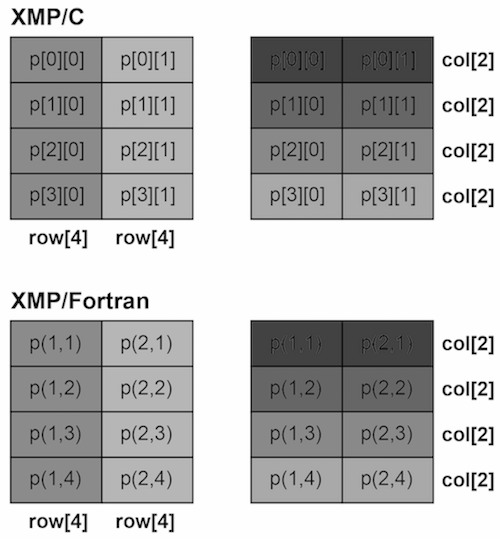
\includegraphics{figs/row_col.png}
  \caption{Partial node set.}
  \label{fig:partial}
\end{figure}

In XMP/C, both p[0][0] and p[0][1] will be row[0]. Likewise, p[0][0],
p[1][0], p[2][0] and p[3][0] will be col[0] in each execution
context. In XMP/Fortran, both p(1,1) and p(2,1) will be
row(1). Likewise, p(1,1), p(1,2), p(1,3) and p(1,4) will be col(1) in
each context.

\begin{mynote}
The syntactic meaning of asterisk symbols in the
node set references are different when declaring a node set and regular
expressions in on clauses.
\end{mynote}


\subsection{{\tt template} Directive}

The template directive declares the name of a template and its
shape. Templates are virtual arrays which used for data and work
mapping. They can have multi-dimensional shapes.

\subsubsection{One-dimensional Template}

\begin{XCexample}
#pragma xmp template t[10]
\end{XCexample}

\begin{XFexample}
!$xmp template t(10)
\end{XFexample}

The template directive declares 1-dimensional template t which has 10
elements. In XMP/C, each element has an unique index from t[0] to
t[9]. Likewise, in XMP/Fortran, the index starts from t(1) to t(10).

\begin{myhint}
In general, the user declare templates which has the same
size with the target data array where data/work mapping is done.
\end{myhint}

In XMP/Fortran, the start index of the template can be given by an
arbitrary number to match the starting array index in the base
language.

\begin{XFexample}
!$xmp template t(-5:4)
\end{XFexample}

The template directive declares 1-dimensional template t starting from t(-5) to t(4).

\begin{mynote}
In XMP/C, templates should start from 0 since array indices
start from 0 in the C language.
\end{mynote}

\subsubsection{Multi-dimensional Template}

\begin{XCexample}
#pragma xmp template t[10][20]
\end{XCexample}

\begin{XFexample}
!$xmp template t(20,10)
\end{XFexample}

The template directive declares 2-dimensional template t which has 10x20
elements. In XMP/C, the template has elements starting from t[0][0] to
t[9][19]. Likewise, the template has elements starting from t(1,1) to
t(20,10) in XMP/Fortran.

\subsubsection{Dynamic Template}

\begin{XCexample}
#pragma xmp template t[:]
\end{XCexample}

\begin{XFexample}
!$xmp template t(:)
\end{XFexample}

A colon symbol is used instead of a number to declare 1-dimensional
dynamic template t. The colon symbol indicates that the size of the
template is undefined. The size of the template is determined at runtime
by {\tt template\_fix} construct.


\subsection{{\tt distribute} Directive}

The distribute directive specifies a distribution of the target
template. The user can specify block, cyclic, block-cyclic, gblock
(irregular data distribution) distribution, which can be chosen by the
target application.

\subsubsection{block distribution}

\begin{XCexample}
#pragma xmp distribute t[block] onto p
\end{XCexample}

\begin{XFexample}
!$xmp distribute t(block) onto p
\end{XFexample}

Target data is divided into contiguous blocks and distributed among
nodes. When the size of the template is N and the number of nodes is K,
the chunk size of each block will be ceil(N/K). For example, block
distribution is useful for stencil computation which refers to
neighborhood elements.

\begin{mynote}
Function ceil(x) returns the minimum integer value which is
greater than x.
\end{mynote}

\begin{XCexample}
#pragma xmp nodes p[3]
#pragma xmp template t[22]
#pragma xmp distribute t[block] onto p
\end{XCexample}

\begin{XFexample}
!$xmp nodes p(3)
!$xmp template t(22)
!$xmp distribute t(block) onto p
\end{XFexample}

\begin{figure}
  \centering
  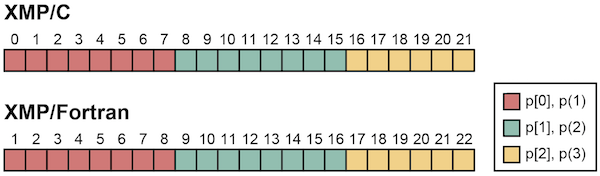
\includegraphics{figs/block.png}
\end{figure}

Since ceil(22/3) is 8, 8 elements will be allocated on p[0] and
p[1]. And then, 6 elements will be allocated on p[2].

The user can specify the size of the block chunk explicitly. In that
case, the remaining elements will be allocated on the last node.

\begin{XCexample}
#pragma xmp nodes p[3]
#pragma xmp template t[22]
#pragma xmp distribute t[block(7)] onto p
\end{XCexample}

\begin{XFexample}
!$xmp nodes p(3)
!$xmp template t(22)
!$xmp distribute t(block(7)) onto p
\end{XFexample}

\begin{figure}
  \centering
  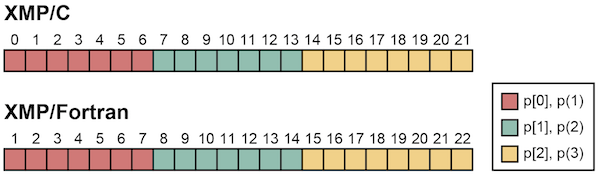
\includegraphics{figs/block2.png}
\end{figure}

Seven elements will be allocated on the p[0] and p[1], as specified in
the directive. And then remaining 8 elements will be allocated on the
last node p[2].

\subsubsection{Cyclic Distribution}

\begin{XCexample}
#pragma xmp distribute t[cyclic] onto p
\end{XCexample}

\begin{XFexample}
!$xmp distribute t(cyclic) onto p
\end{XFexample}

Target data is divided into a chunk of a single element and distributed
among nodes in a round-robin manner. Cyclic distribution is suitable for
computation with an irregular load balance of data and computation.

\begin{XCexample}
#pragma xmp nodes p[3]
#pragma xmp template t[22]
#pragma xmp distribute t[cyclic] onto p
\end{XCexample}

\begin{XFexample}
!$xmp nodes p(3)
!$xmp template t(22)
!$xmp distribute t(cyclic) onto p
\end{XFexample}

\begin{figure}
  \centering
  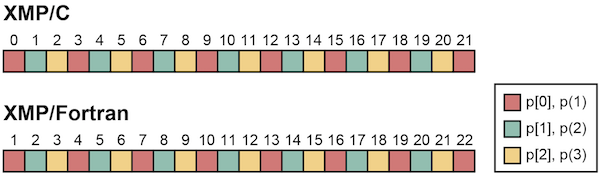
\includegraphics{figs/cyclic.png}
\end{figure}

\subsubsection{Block-cyclic Distribution}

\begin{XCexample}
#pragma xmp distribute t[cyclic(w)] onto p
\end{XCexample}

\begin{XFexample}
!$xmp distribute t(cyclic(w)) onto p
\end{XFexample}

Target data is divided into a contiguous block of size w and distributed
among nodes in a round-robin manner. Block-cyclic distribution is
suitable for computation which has an irregular load balance and
references to neighborhood elements.

\begin{XCexample}
#pragma xmp nodes p[3]
#pragma xmp template t[22]
#pragma xmp distribute t[cyclic(3)] onto p
\end{XCexample}

\begin{XFexample}
!$xmp nodes p(3)
!$xmp template t(22)
!$xmp distribute t(cyclic(3)) onto p
\end{XFexample}

\begin{figure}
  \centering
  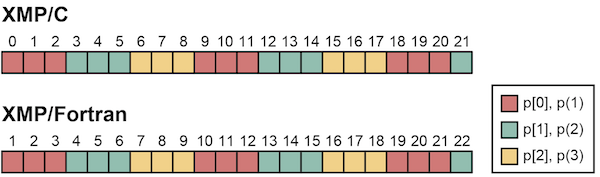
\includegraphics{figs/block-cyclic.png}
\end{figure}

\subsubsection{Gblock Distribution}

\begin{XCexample}
#pragma xmp distribute t[gblock(W)] onto p
\end{XCexample}

\begin{XFexample}
!$xmp distribute t(gblock(W)) onto p
\end{XFexample}

Array W is a mapping array which is used for irregular data
distribution. W[k]/W(k) elements will be allocated on node p(k). The
user can specify a special type of data distribution explicitly by using
mapping arrays (e.g. distribution of triangular matrix).

\begin{XCexample}
#pragma xmp nodes p[3]
#pragma xmp template t[22]
int W[3] = {6, 11, 5};
#pragma xmp distribute t[gblock(W)] onto p
\end{XCexample}

\begin{XFexample}
!$xmp nodes p(3)
!$xmp template t(22)
integer, parameter :: W(3) = (/6,11,5/)
!$xmp distribute t(gblock(W)) onto p
\end{XFexample}

\begin{figure}
  \centering
  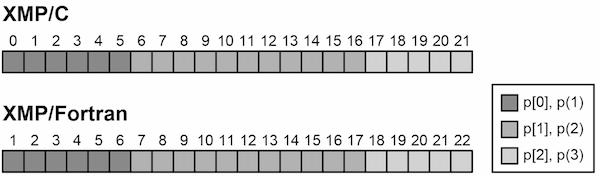
\includegraphics{figs/gblock.png}
\end{figure}

The user can specify an asterisk symbol instead of a mapping array in
gblock. In that case, data distribution will be determined at runtime by
using {\tt template\_fix} construct.

\subsubsection{Distribution of Multi-dimensional Template}

The user can distribute a multi-dimensional template with a
(single-/multi-dimensional) node set.

\begin{XCexample}
#pragma xmp nodes p[2][2]
#pragma xmp template t[10][10]
#pragma xmp distribute t[block][block] onto p
\end{XCexample}

\begin{XFexample}
!$xmp nodes p(2,2)
!$xmp template t(10,10)
!$xmp distribute t(block,block) onto p
\end{XFexample}

The distribute directive declares data distribution of a 2-dimensional
template by using a 2-dimensional node set. Each dimension of the
template is divided by block distribution on a node set p.

\begin{figure}
  \centering
  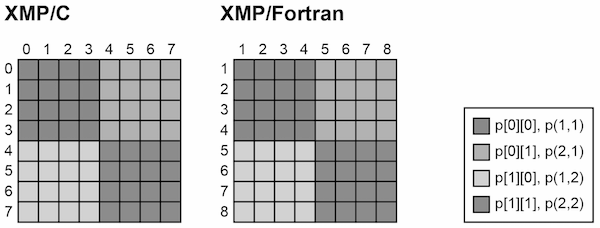
\includegraphics{figs/multi.png}
\end{figure}

The user can specify a different distribution pattern to each dimension.

\begin{XCexample}
#pragma xmp nodes p[2][2]
#pragma xmp template t[10][10]
#pragma xmp distribute t[block][cyclic] onto p
\end{XCexample}

\begin{XFexample}
!$xmp nodes p(2,2)
!$xmp template t(10,10)
!$xmp distribute t(cyclic,block) onto p
\end{XFexample}

\begin{figure}
  \centering
  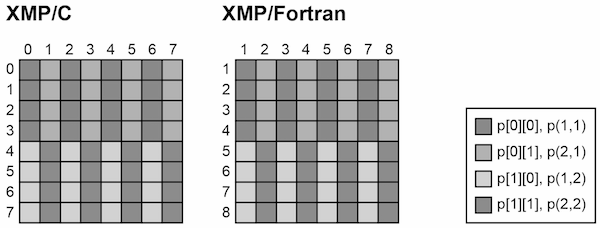
\includegraphics{figs/multi2.png}
\end{figure}

When an asterisk symbol is given in the distribute directive instead of
distribution type, the target dimension will remain undistributed. In
the following example, the first dimension will be distributed in a
block manner and the second dimension will remain undistributed.

\begin{XCexample}
#pragma xmp nodes p[4]
#pragma xmp template t[10][10]
#pragma xmp distribute t[block][*] onto p
\end{XCexample}

\begin{XFexample}
!$xmp nodes p(4)
!$xmp template t(10,10)
!$xmp distribute t(*,block) onto p
\end{XFexample}

\begin{figure}
  \centering
  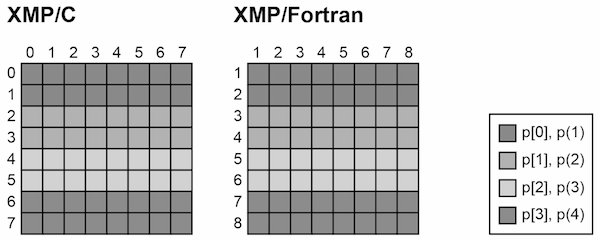
\includegraphics{figs/multi3.png}
\end{figure}

\subsection{{\tt align} Directive}

The align directive performs data mapping and distributes data among
nodes by using a distributed template. The align directive should be
given after the target array definition.

\subsubsection{Normal Alignment}

\begin{XCexample}
#pragma xmp nodes p[4]
#pragma xmp template t[8]
#pragma xmp distribute t[block] onto p
int a[8];
#pragma xmp align a[i] with t[i]
\end{XCexample}

\begin{XFexample}
!$xmp nodes p(4)
!$xmp template t(8)
!$xmp distribute t(block) onto p
integer :: a(8)
!$xmp align a(i) with t(i)
\end{XFexample}

The align directive aligns the owner node of a[i] with t(i), a
distributed template. As a result, array a is distributed among the node
set p.

\begin{figure}
  \centering
  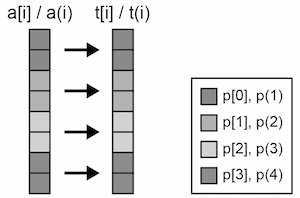
\includegraphics{figs/1dim.png}
\end{figure}

The align directive also can be used for multi-dimensional arrays.

\begin{XCexample}
#pragma xmp nodes p[2][2]
#pragma xmp template t[8][8]
#pragma xmp distribute t[block][block] onto p
int a[8][8];
#pragma xmp align a[i][j] with t[i][j]
\end{XCexample}

\begin{XFexample}
!$xmp nodes p(2,2)
!$xmp template t(8,8)
!$xmp distribute t(block,block) onto p
integer :: a(8,8)
!$xmp align a(j,i) with t(j,i)
\end{XFexample}

\begin{figure}
  \centering
  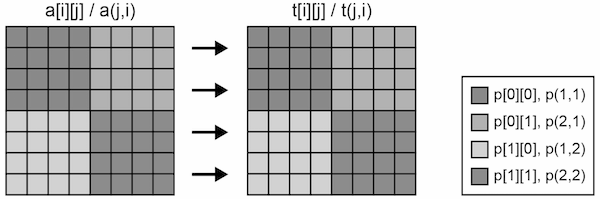
\includegraphics{figs/multi-dim.png}
\end{figure}

\subsubsection{Special Alignment}

\paragraph{Collapse}

The user can align a 2-dimensional array with a 1-dimensional template.

\begin{XCexample}
#pragma xmp nodes p[4]
#pragma xmp template t[8]
#pragma xmp distribute t[block] onto p
int a[8][8];
#pragma xmp align a[i][*] with t[i]
\end{XCexample}

\begin{XFexample}
!$xmp nodes p(4)
!$xmp template t(8)
!$xmp distribute t(block) onto p
integer :: a(8,8)
!$xmp align a(*,i) with t(i)
\end{XFexample}

When an asterisk symbol is given in the array reference in the align
directive, the specified dimension is not distributed among the node
set. In the sample program, the first dimension of the array a is
distributed among node set p while the second dimension is duplicated.

\begin{figure}
  \centering
  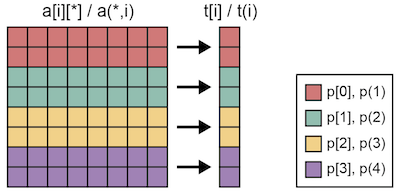
\includegraphics{figs/collapse.png}
\end{figure}

In XMP/C, a[0:2][:] will be allocated on p[0]. Likewise, a(:,1:2) will
be allocated on p(1) in XMP/Fortran.

\paragraph{Replicate}

The user also can align a 1-dimensional array with a multi-dimensional
template.

\begin{XCexample}
#pragma xmp nodes p[2][2]
#pragma xmp template t[8][8]
#pragma xmp distribute t[block][block] onto p
int a[8];
#pragma xmp align a[i] with t[i][*]
\end{XCexample}

\begin{XFexample}
!$xmp nodes p(2,2)
!$xmp template t(8,8)
!$xmp distribute t(block,block) onto p
integer :: a(8)
!$xmp align a(i) with t(*,i)
\end{XFexample}

When an asterisk symbol is given in the template reference in the align
directive, the owner nodes of the specified dimension will have
duplicated elements of the target array.

\begin{figure}
  \centering
  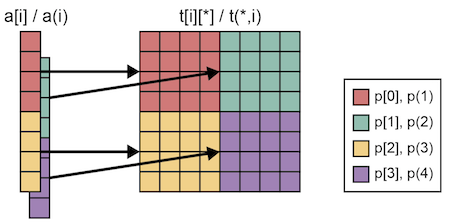
\includegraphics{figs/replicate.png}
\end{figure}

In XMP/C, a[0:4] will be duplicated and allocated on p[0][0] and
  p[0][1]. Likewise, a(1:4) will be allocated on p(1,1) and p(2,1) in
  XMP/Fortran.



% \subsection{Dynamic Allocation of Distributed Array}

% This section explains how distributed arrays are allocated at
% runtime. The basic procedure is common in XMP/C and XMP/Fortran with a
% few specific difference.

% \subsubsection{One-dimensional Array}

% \begin{XCexample}
% #pragma xmp nodes p[4]
% #pragma xmp template t[N]
% #pragma xmp distribute t[block] onto p
% float *a;
% #pragma xmp align a[i] with t[i]
%   :
% a = xmp_malloc(xmp_desc_of(a), N);
% \end{XCexample}

% First, declare a pointer of the type of the target distributed
% array. Second, align it as if it were an array. Finally, allocate memory
% for it with the {\tt xmp\_malloc()} function. {\tt xmp\_desc\_of()} is an
% intrinsic/builtin function that returns the descriptor of the XMP object
% specified by the argument.

% \begin{XFexample}
% !$xmp nodes p(4)
% !$xmp template t(N)
% !$xmp distribute t(block) onto p
% real, allocatable :: a(:)
% !$xmp align a(i) with t(i)

% allocate(a(N))
% \end{XFexample}

% First, declare an allocatable array of the type of the target
% distributed array. Second, align it. Finally, allocate memory for it
% with the allocate statement.

% \subsubsection{Multi-dimensional Array}

% The procedure is the same as that for a one-dimensional array.

% \begin{XCexample}
% #pragma xmp nodes p[2][2]
% #pragma xmp template t[N1][N2]
% #pragma xmp distribute t[block][block] onto p
% float (*a)[N2];
% #pragma xmp align a[i][j] with t[i][j]
%   :
% a = (float (*)[N2])xmp_malloc(xmp_desc_of(a), N1, N2);
% \end{XCexample}

% \begin{XFexample}
% !$xmp nodes p(2,2)
% !$xmp template t(N2,N1)
% !$xmp distribute t(block,block) onto p
% real, allocatable :: a(:,:)
% !$xmp align a(j,i) with t(j,i)
%   :
% allocate(a(N2,N1))
% \end{XFexample}

% \noindent\hrulefill

% {\bf Note}: If the size of template is not fixed until runtime, use
% {\tt template\_fix}
% construct.

% \noindent\hrulefill

\subsection{{\tt template\_fix} Construct}

The {\tt template\_fix} construct defines the size and distribution of an
unfixed template. It is also used when a distributed array is allocated
at runtime.

\begin{XCexample}
#pragma xmp nodes p[4]
#pragma xmp template t[:]
#pragma xmp distribute t[block] onto p
double *a;
#pragma xmp align a[i] with t[i]

int n = 100;
#pragma xmp template_fix t[n]
a = xmp_malloc(xmp_desc_of(a), n);
\end{XCexample}

\begin{XFexample}
!$xmp nodes p(4)
!$xmp template t(:)
!$xmp distribute t(block) onto p
real, allocatable :: a(:)
integer :: n
!$xmp align a(i) with t(i)

n = 100
!$xmp template_fix t(n)
allocate(a(n))
\end{XFexample}

First, declare a template the size of which is undefined using the ”:”
notation. Second, align a pointer in XMP/C and an allocatable array in
XMP/Fortran with the template. Third, fix the size of the template with
a {\tt template\_fix} construct. Finally, allocate the array with the
{\tt xmp\_malloc()} builtin function in XMP/C and the allocate statement in
XMP/Fortran.

\begin{mynote}
{\bf Note}: {\tt template\_fix} constructs can be applied to a template only once.
\end{mynote}

The {\tt template\_fix} construct can also be used to define a mapping array of
a template that is distributed in “gblock(*)” at declaration.

\begin{XCexample}
#pragma xmp nodes p[4]
#pragma xmp template t[:]
#pragma xmp distribute t[gblock(*)] onto p
double *a;
#pragma xmp align a[i] with t[i]

int n = 100;
int m[] = {40,30,20,10};

#pragma xmp template_fix[gblock(m)] t[n]
a = xmp_malloc(xmp_desc_of(a), n);
\end{XCexample}

\begin{XFexample}
!$xmp nodes p(4)
!$xmp template t(:)
!$xmp distribute t(gblock) onto p
real, allocatable :: a(:)
integer :: n, m(4)
!$xmp align a(i) with t(i)

n = 100
m(:) = (/40,30,20,10/)
!$xmp template_fix(gblock(m)) t(n)
allocate(a(n))
\end{XFexample}
